\section{Results} \label{results}

\subsection{Models} \label{results:models}
Multiple models were used to evaluate the implemented methods in section \ref{implementation}. The model with the largest scale is the Disney cloud \cite{DisneyCloud}. Our implementation is bound by volumes with size $4096^3$ so we use the half resolution version. We also use multiple models from the \href{https://www.openvdb.org/download/}{OpenVDB website} and the \href{https://jangafx.com/software/embergen/download/free-vdb-animations/}{JangaFX website}. A mix of models was used with diverse axis size, number of voxels, animation frame number and shapes. 

\begin{table}[htbp]
    \centering 
    \begin{tabularx}{\textwidth}{|X|c|c|c|c|}
    \hline
    \textbf{Model} & \textbf{Voxels} & \textbf{Dimensions} & \textbf{Animation frames} & \textbf{Render}\\
    \hline
    \textbf{fire} & 4,458,790 & [160, 363, 152] & 1 & 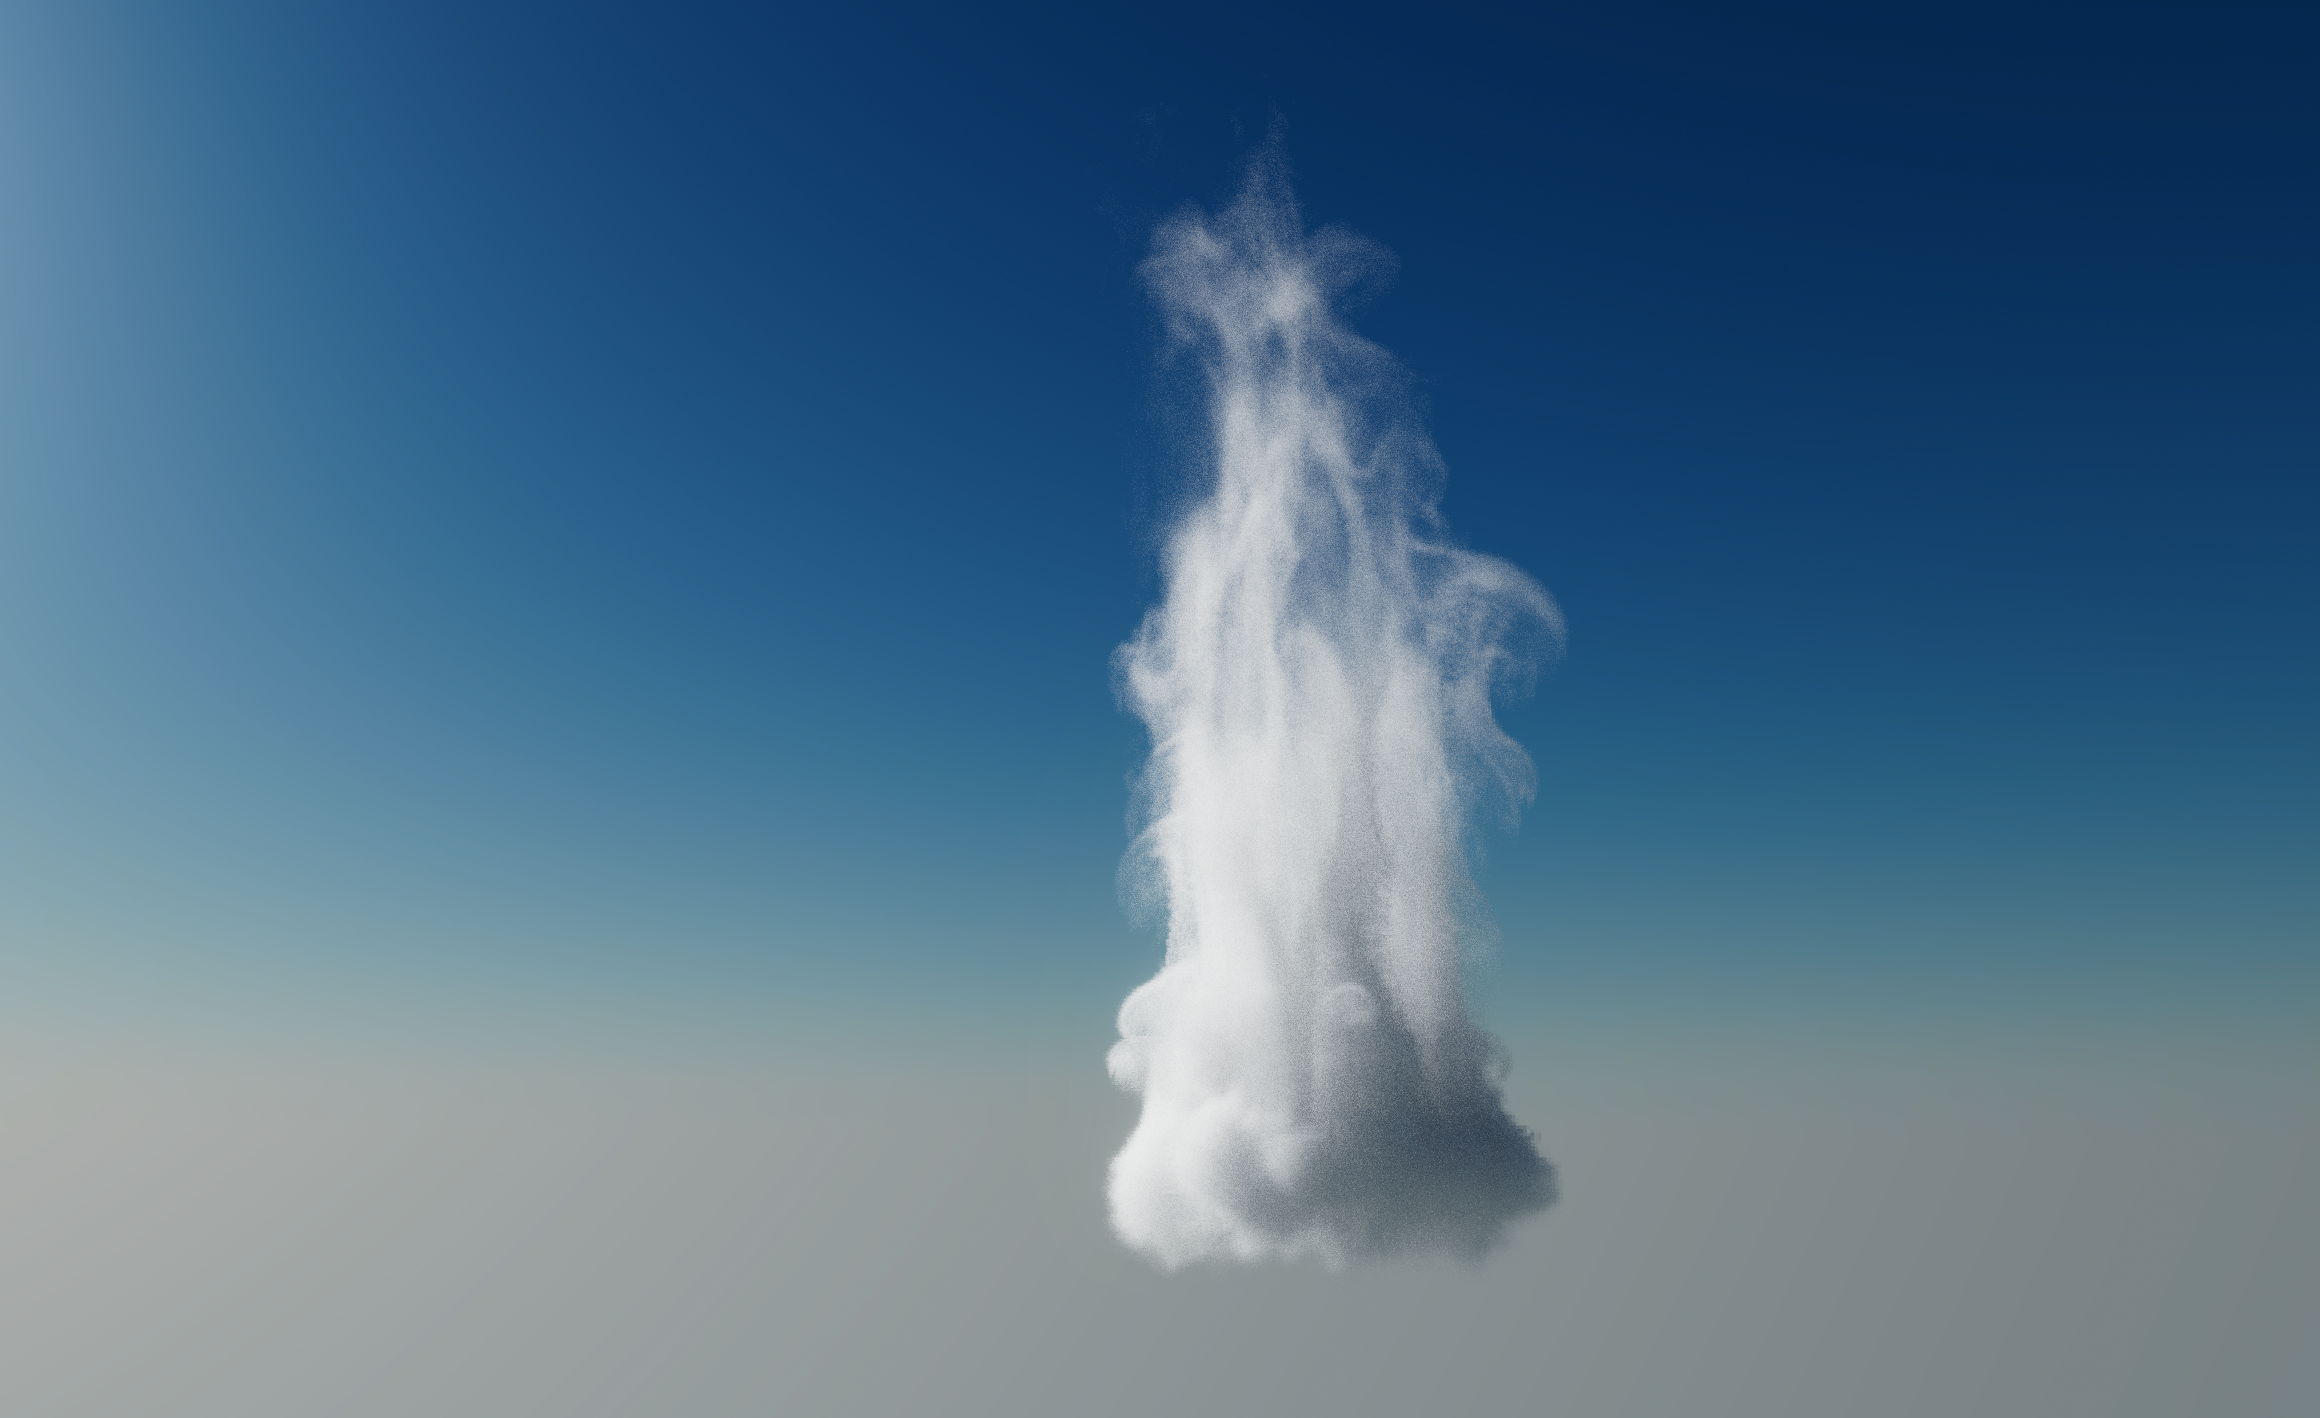
\includegraphics[width=4cm]{figures/fire.png}\\
    \hline
    \textbf{bunny} & 5,513,993 & [627, 620, 488] & 1 & 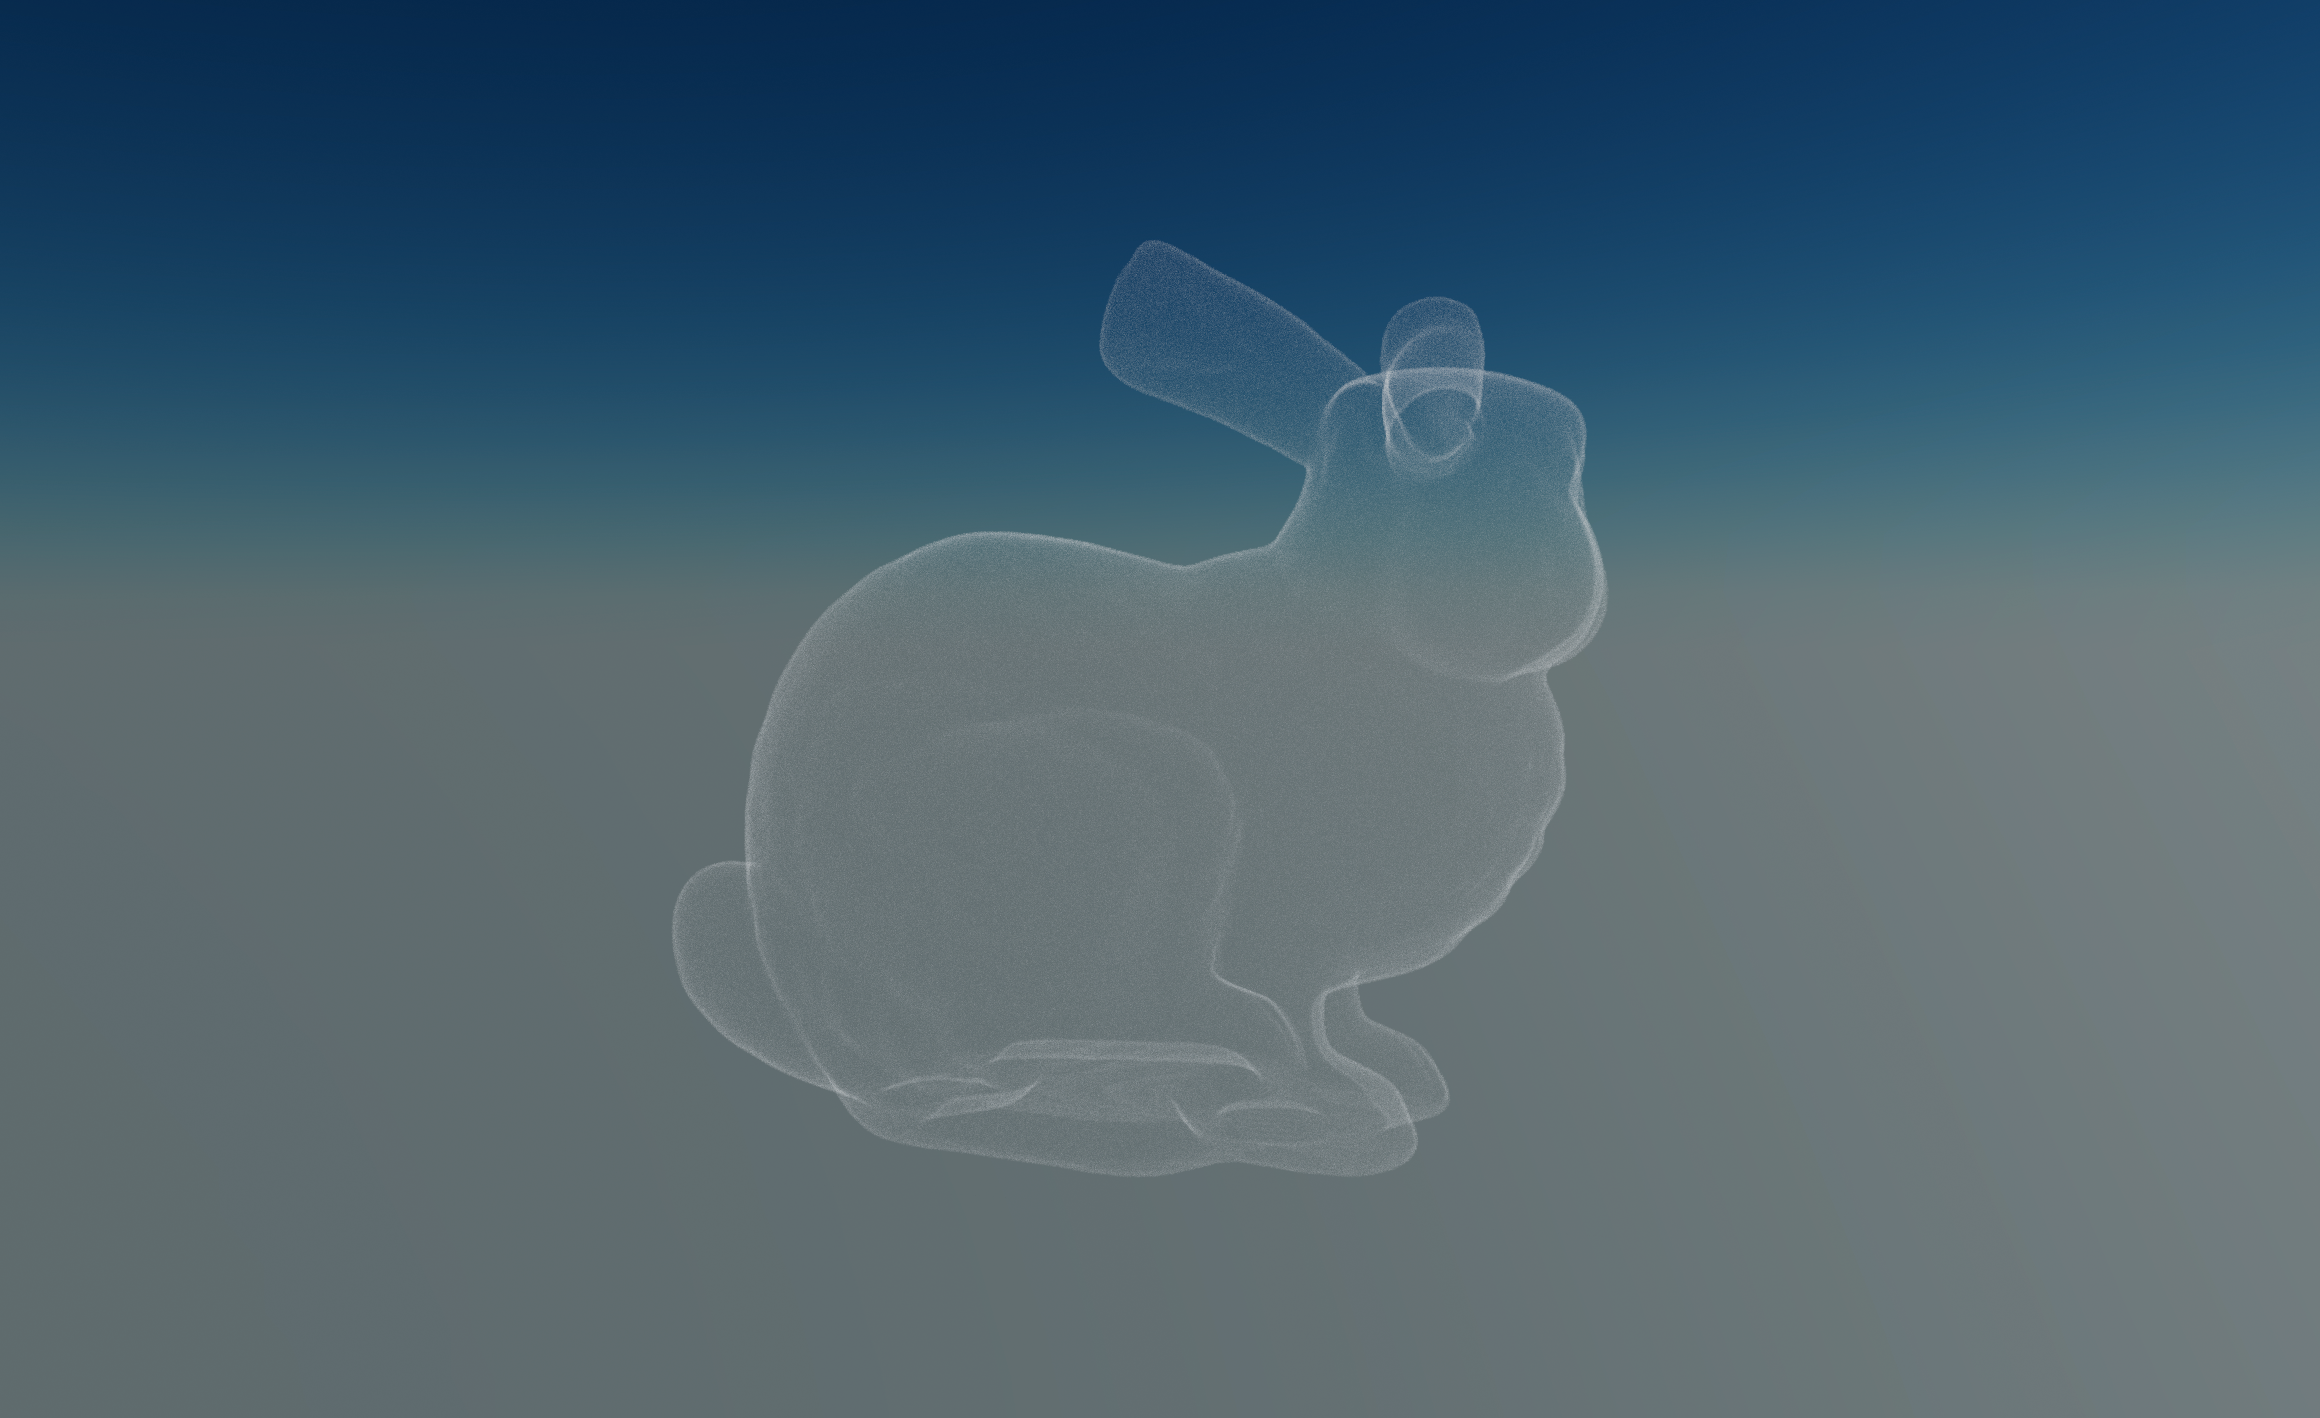
\includegraphics[width=4cm]{figures/bunny.png}\\
    \hline
    \textbf{bunny cloud} & 19,210,271 & [576, 571, 437] & 1 & 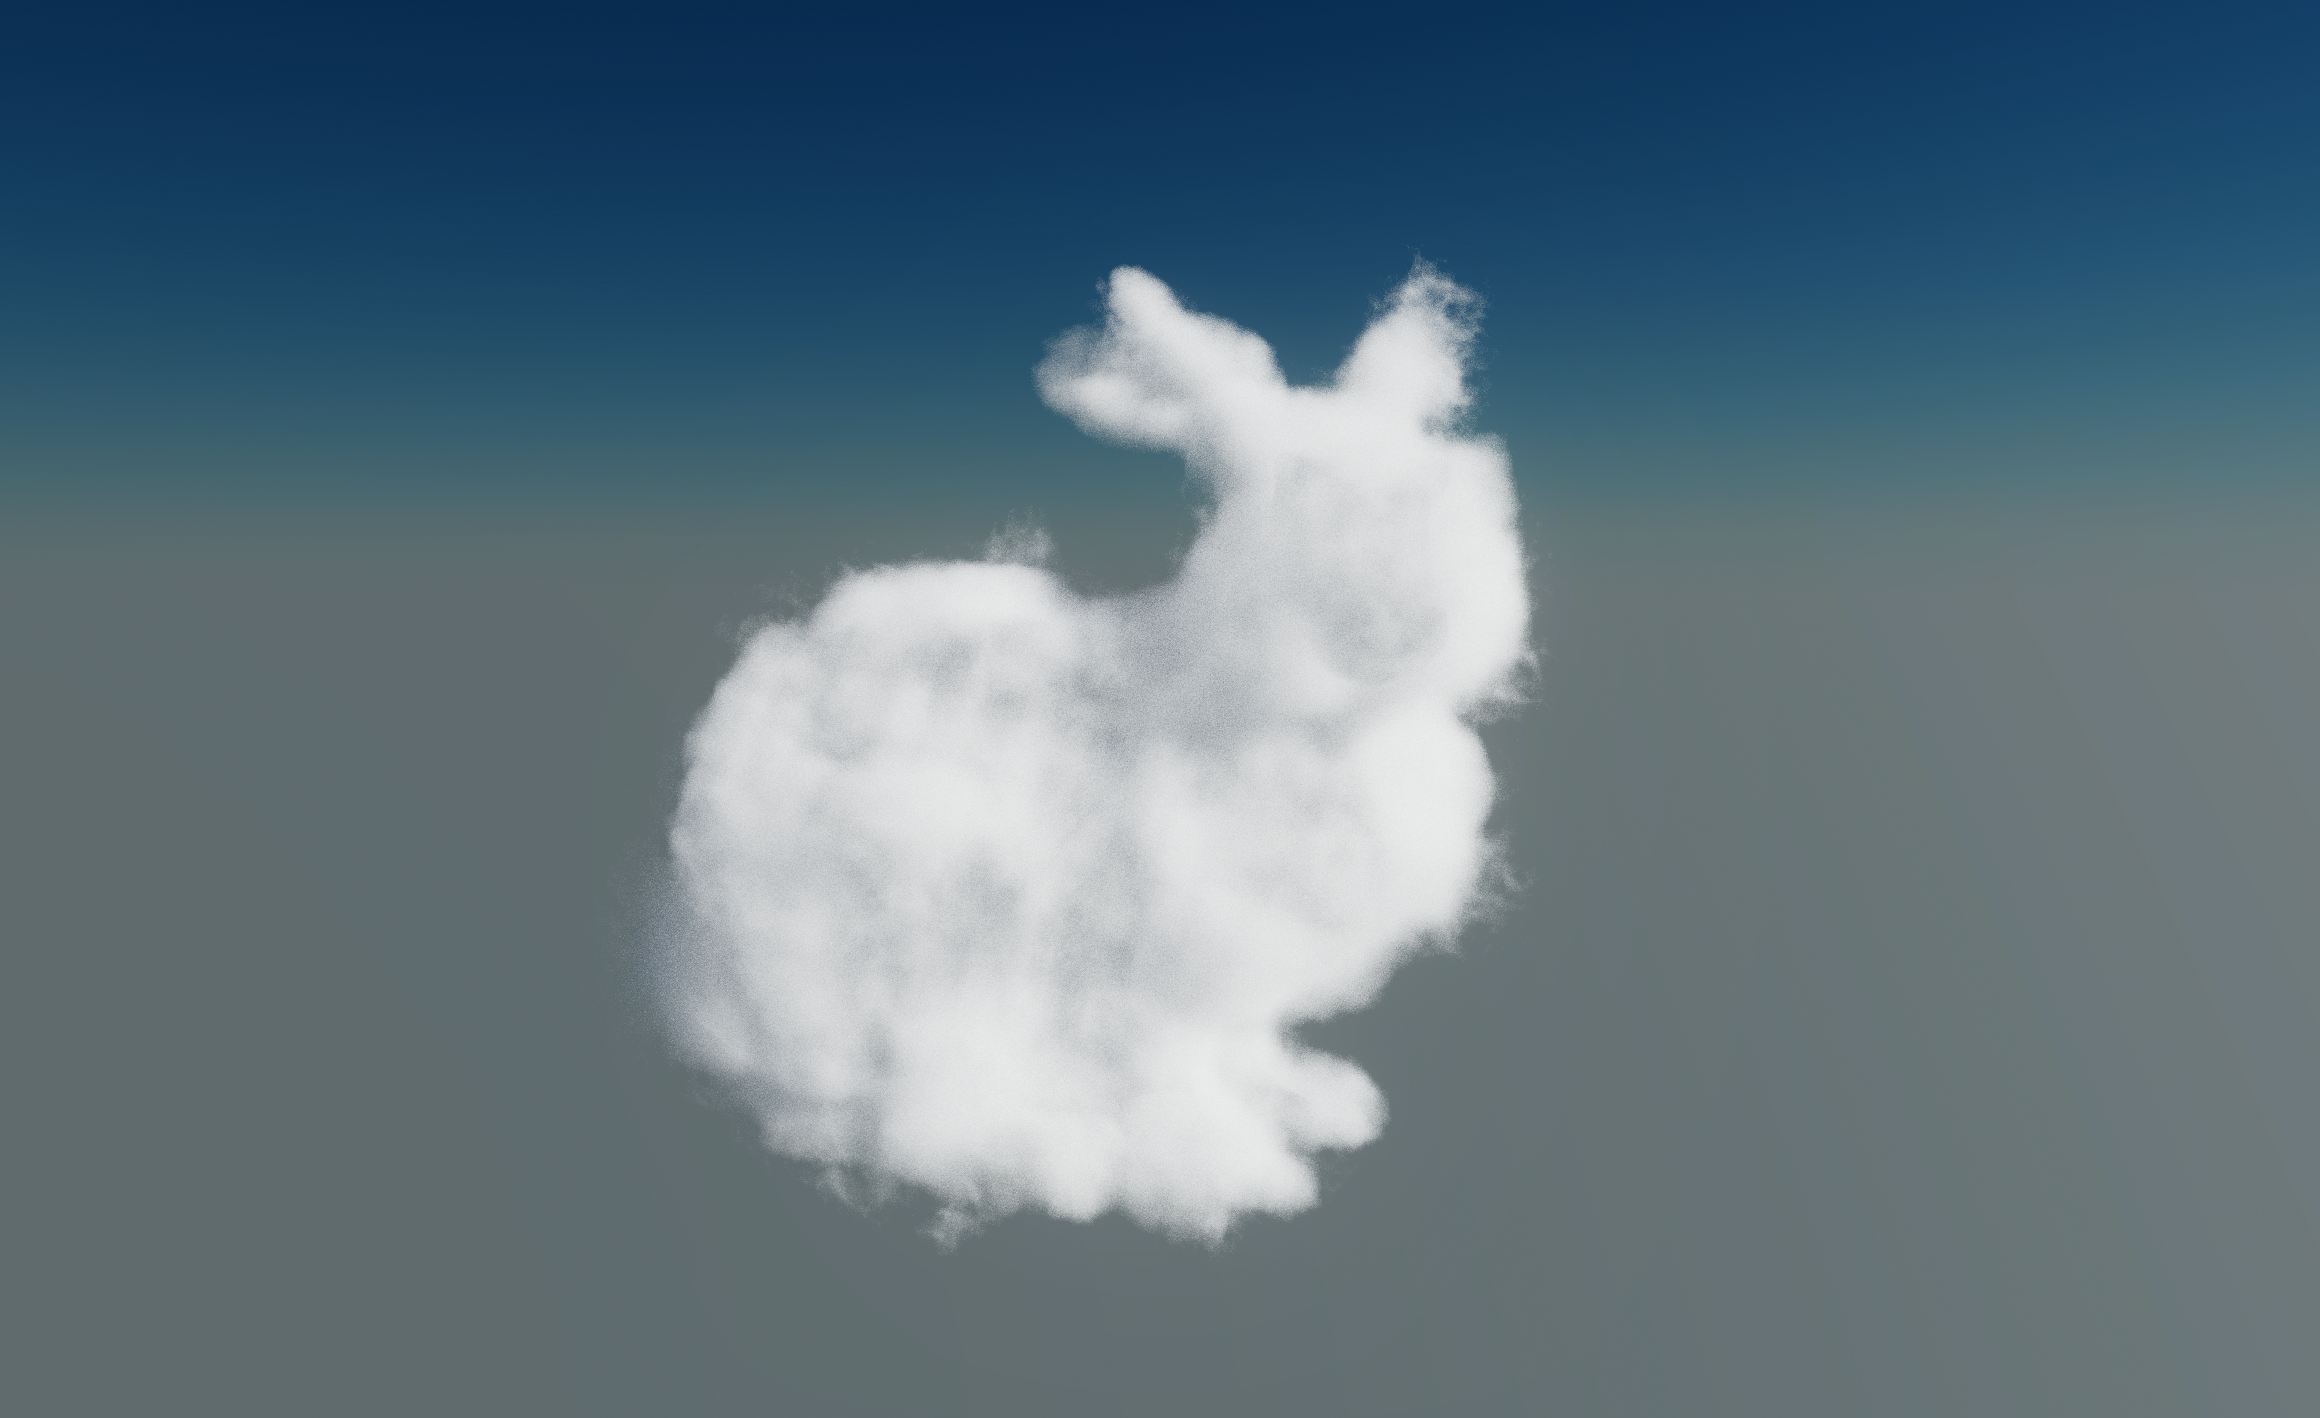
\includegraphics[width=4cm]{figures/bunny cloud.png}\\
    \hline
    \textbf{armadillo} & 22,734,512 & [1,275, 1,518, 1,159] & 1 & 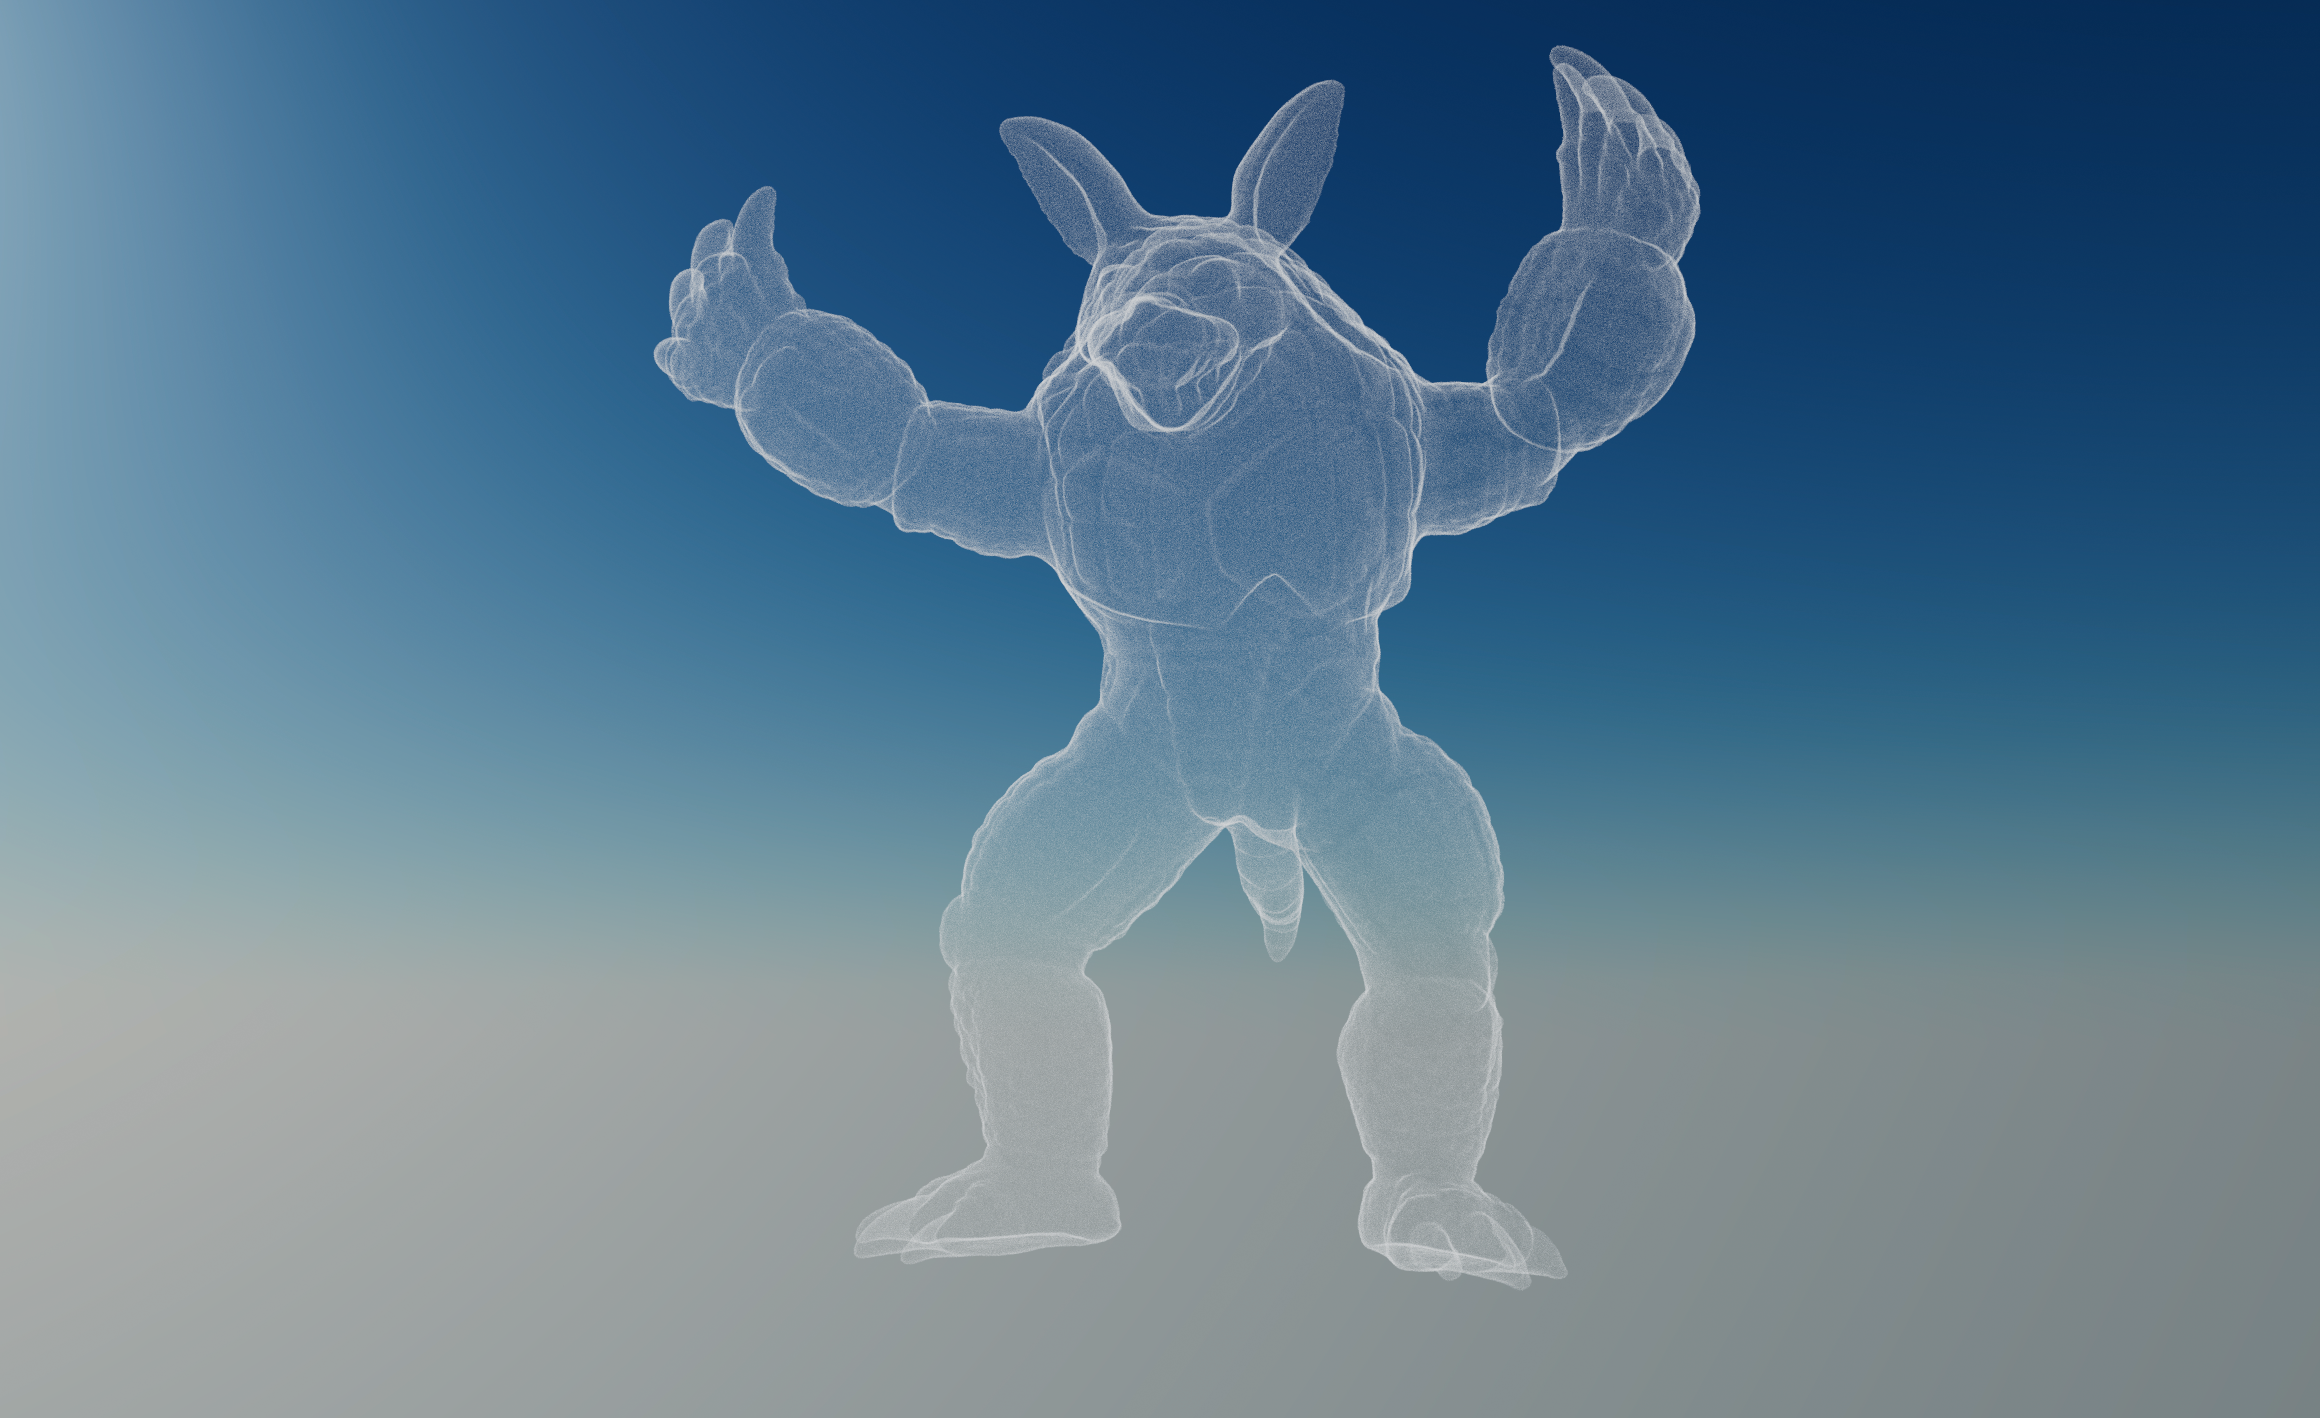
\includegraphics[width=4cm]{figures/armadilo.png}\\
    \hline
    \textbf{dragon} & 23,347,893 & [2,022, 910, 1,346] & 1 & 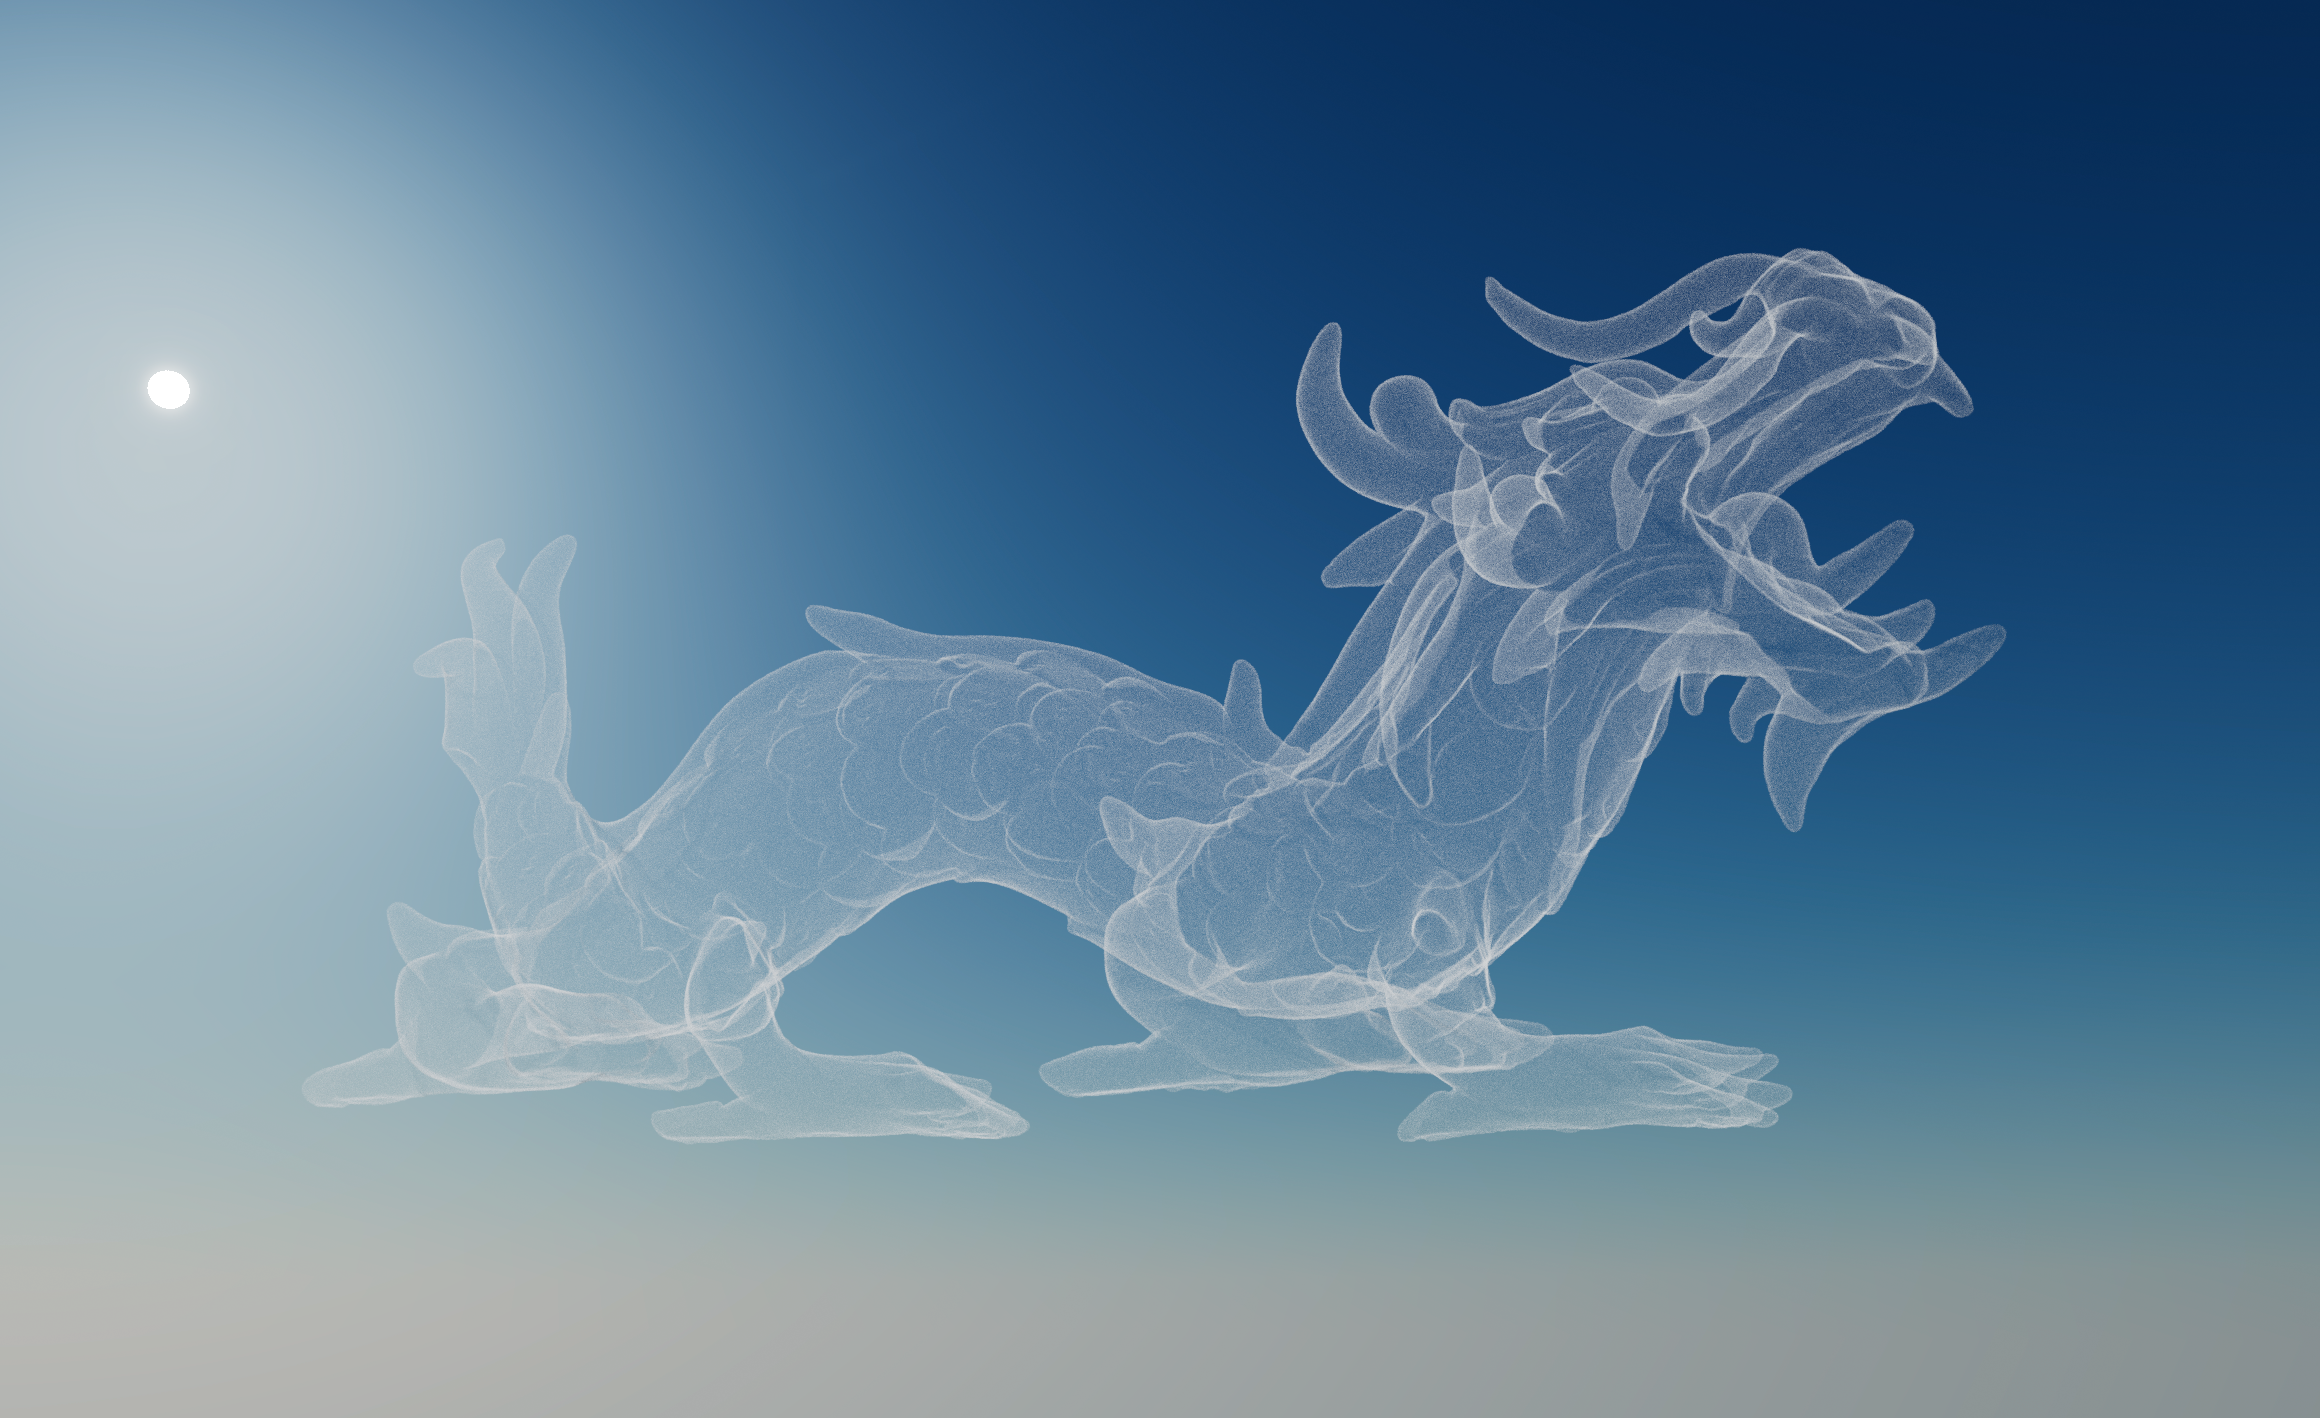
\includegraphics[width=4cm]{figures/dragon.png}\\
    \hline
    \textbf{cloud pack} & 49,869,596 & [349, 178, 530] & 10 & 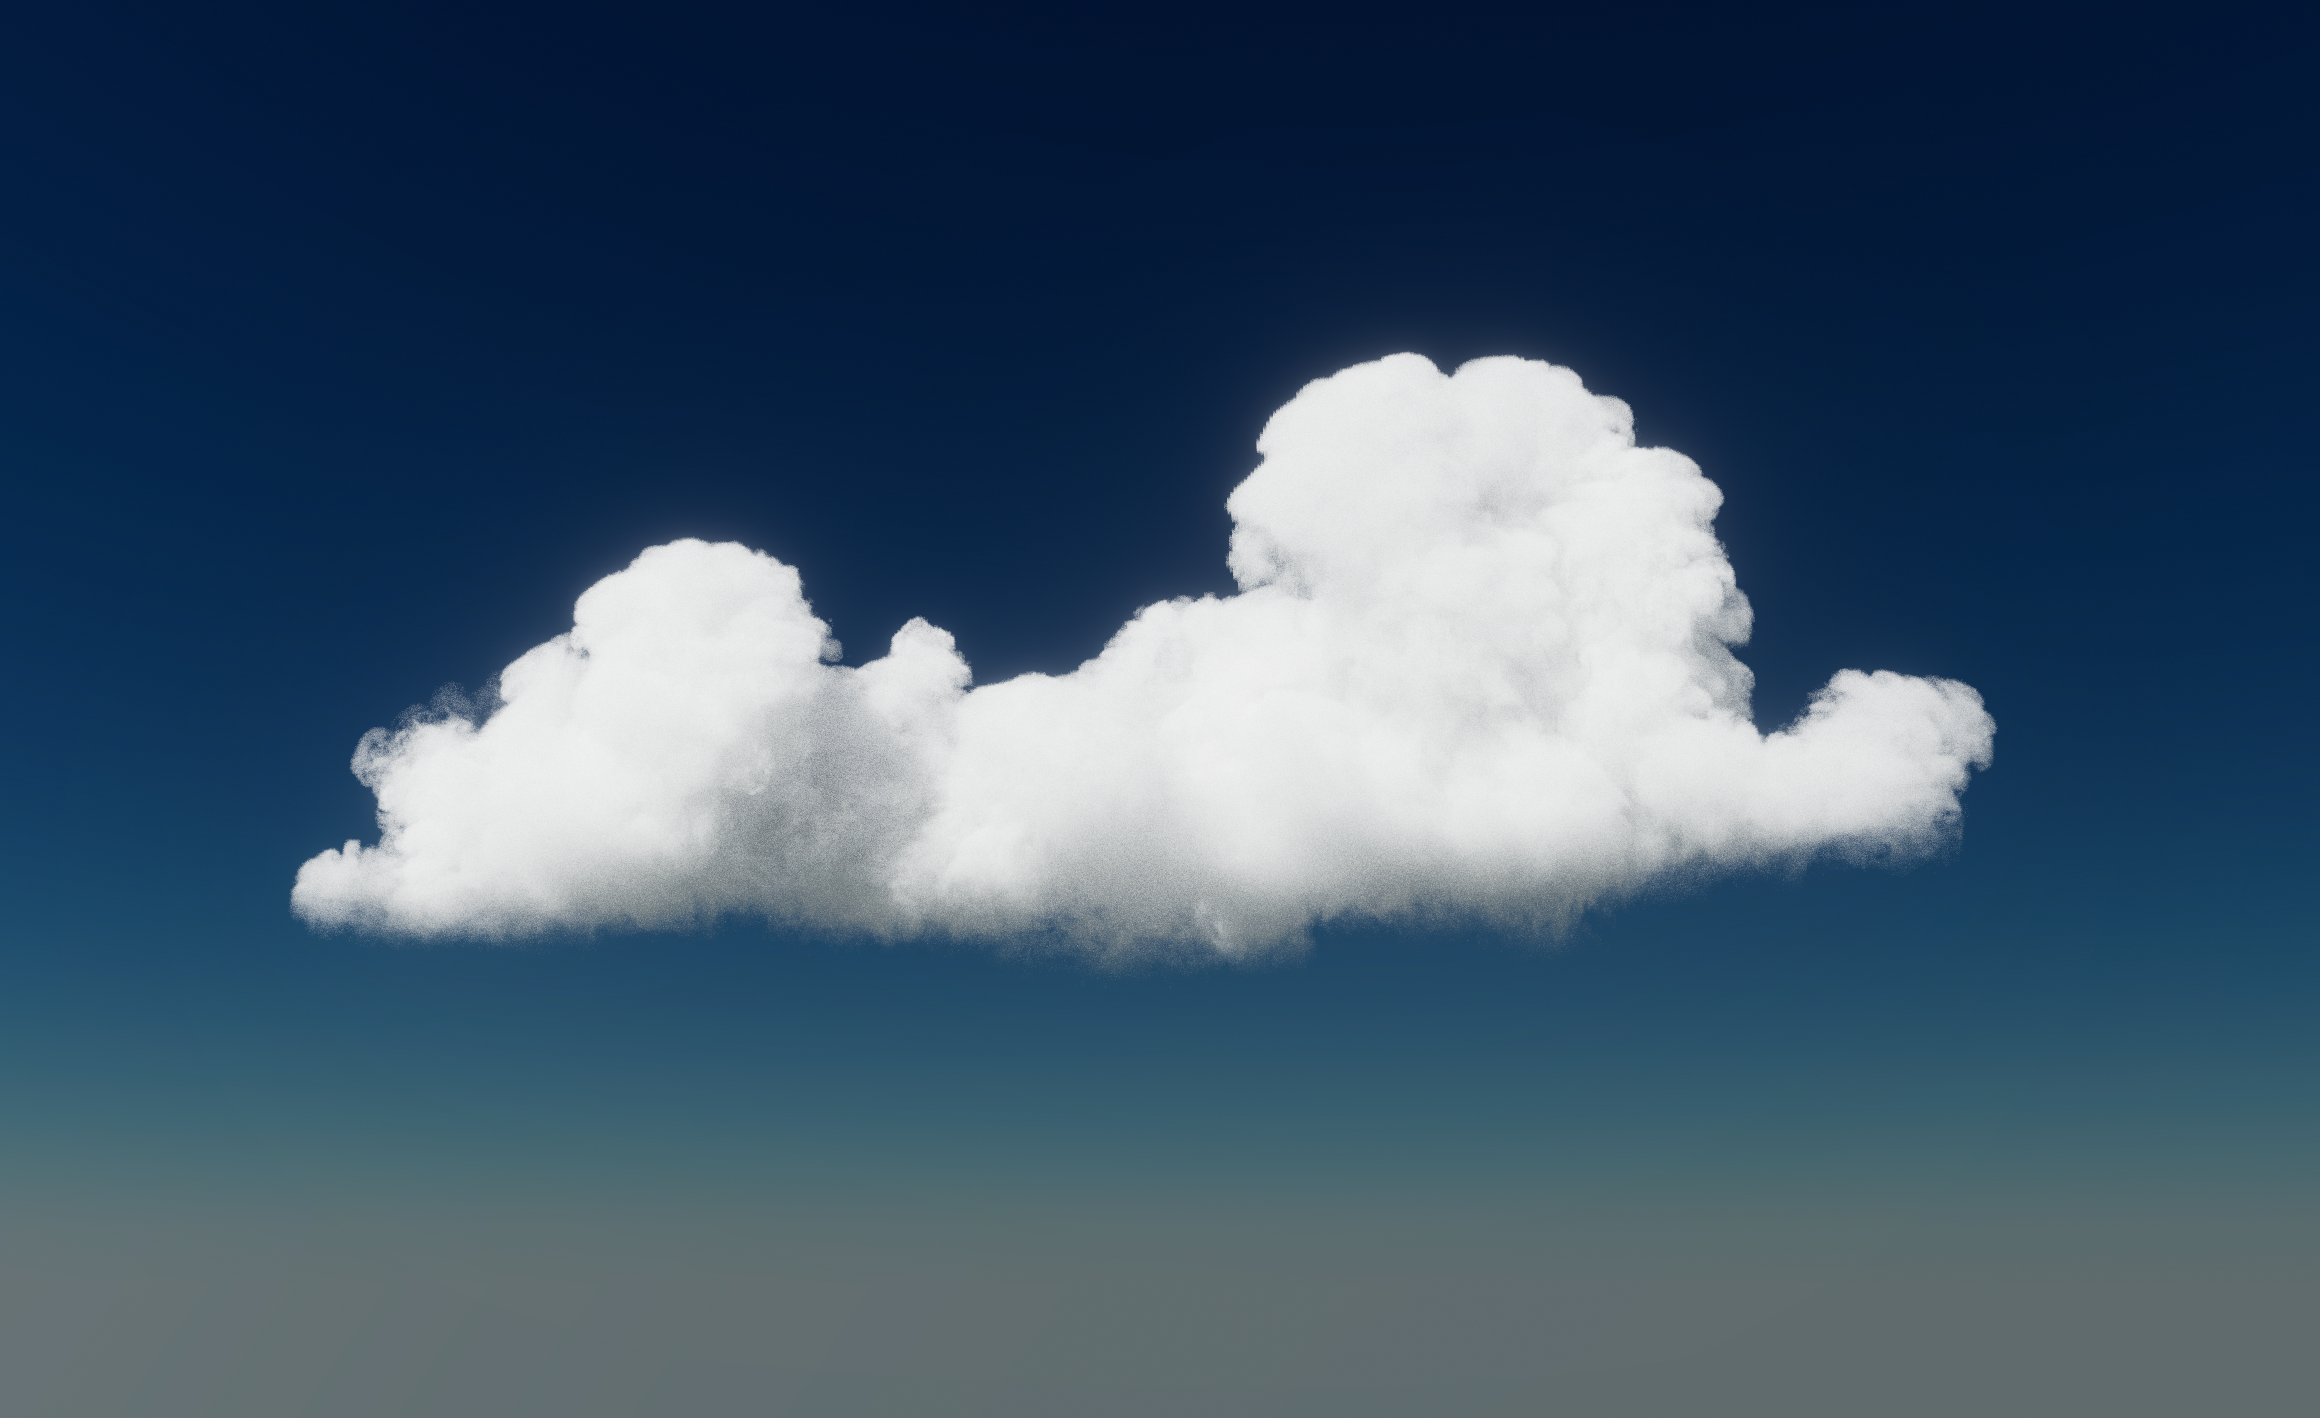
\includegraphics[width=4cm]{figures/cloud pack.png}\\
    \hline
    \raggedright\textbf{disney cloud half res} & 188,358,293 & [993, 675, 1,224] & 1 & 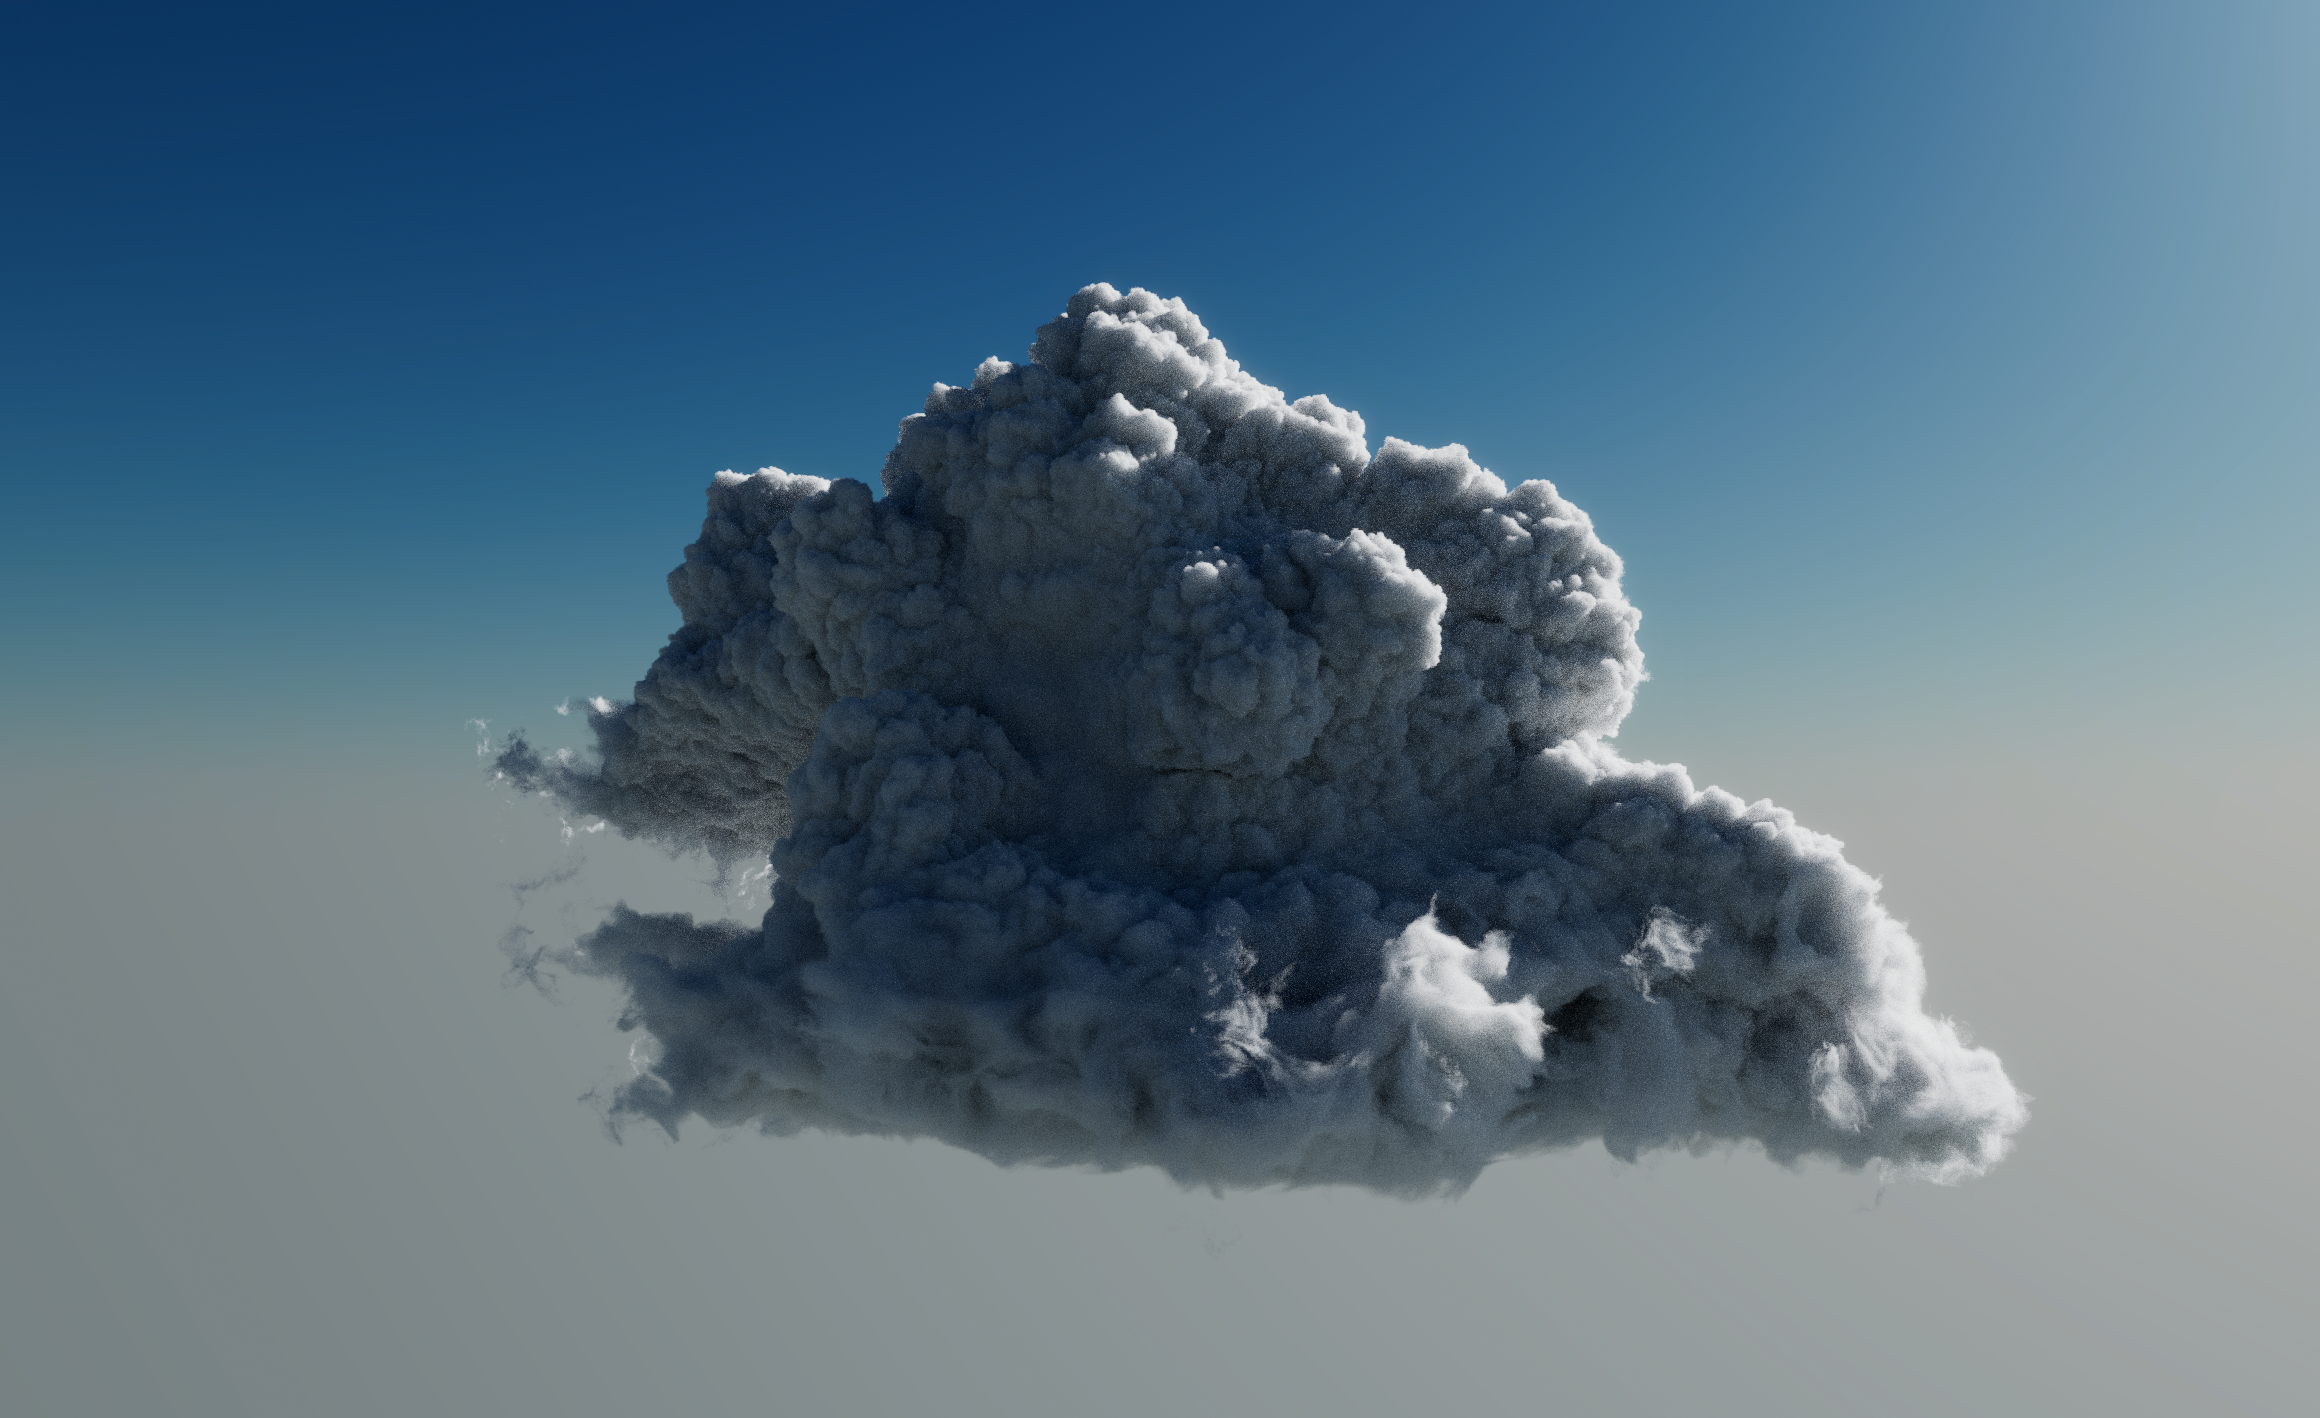
\includegraphics[width=4cm]{figures/disney cloud.png}\\
    \hline
    \textbf{chimney} & 239,747,485 & [160, 350, 505] & 100 & 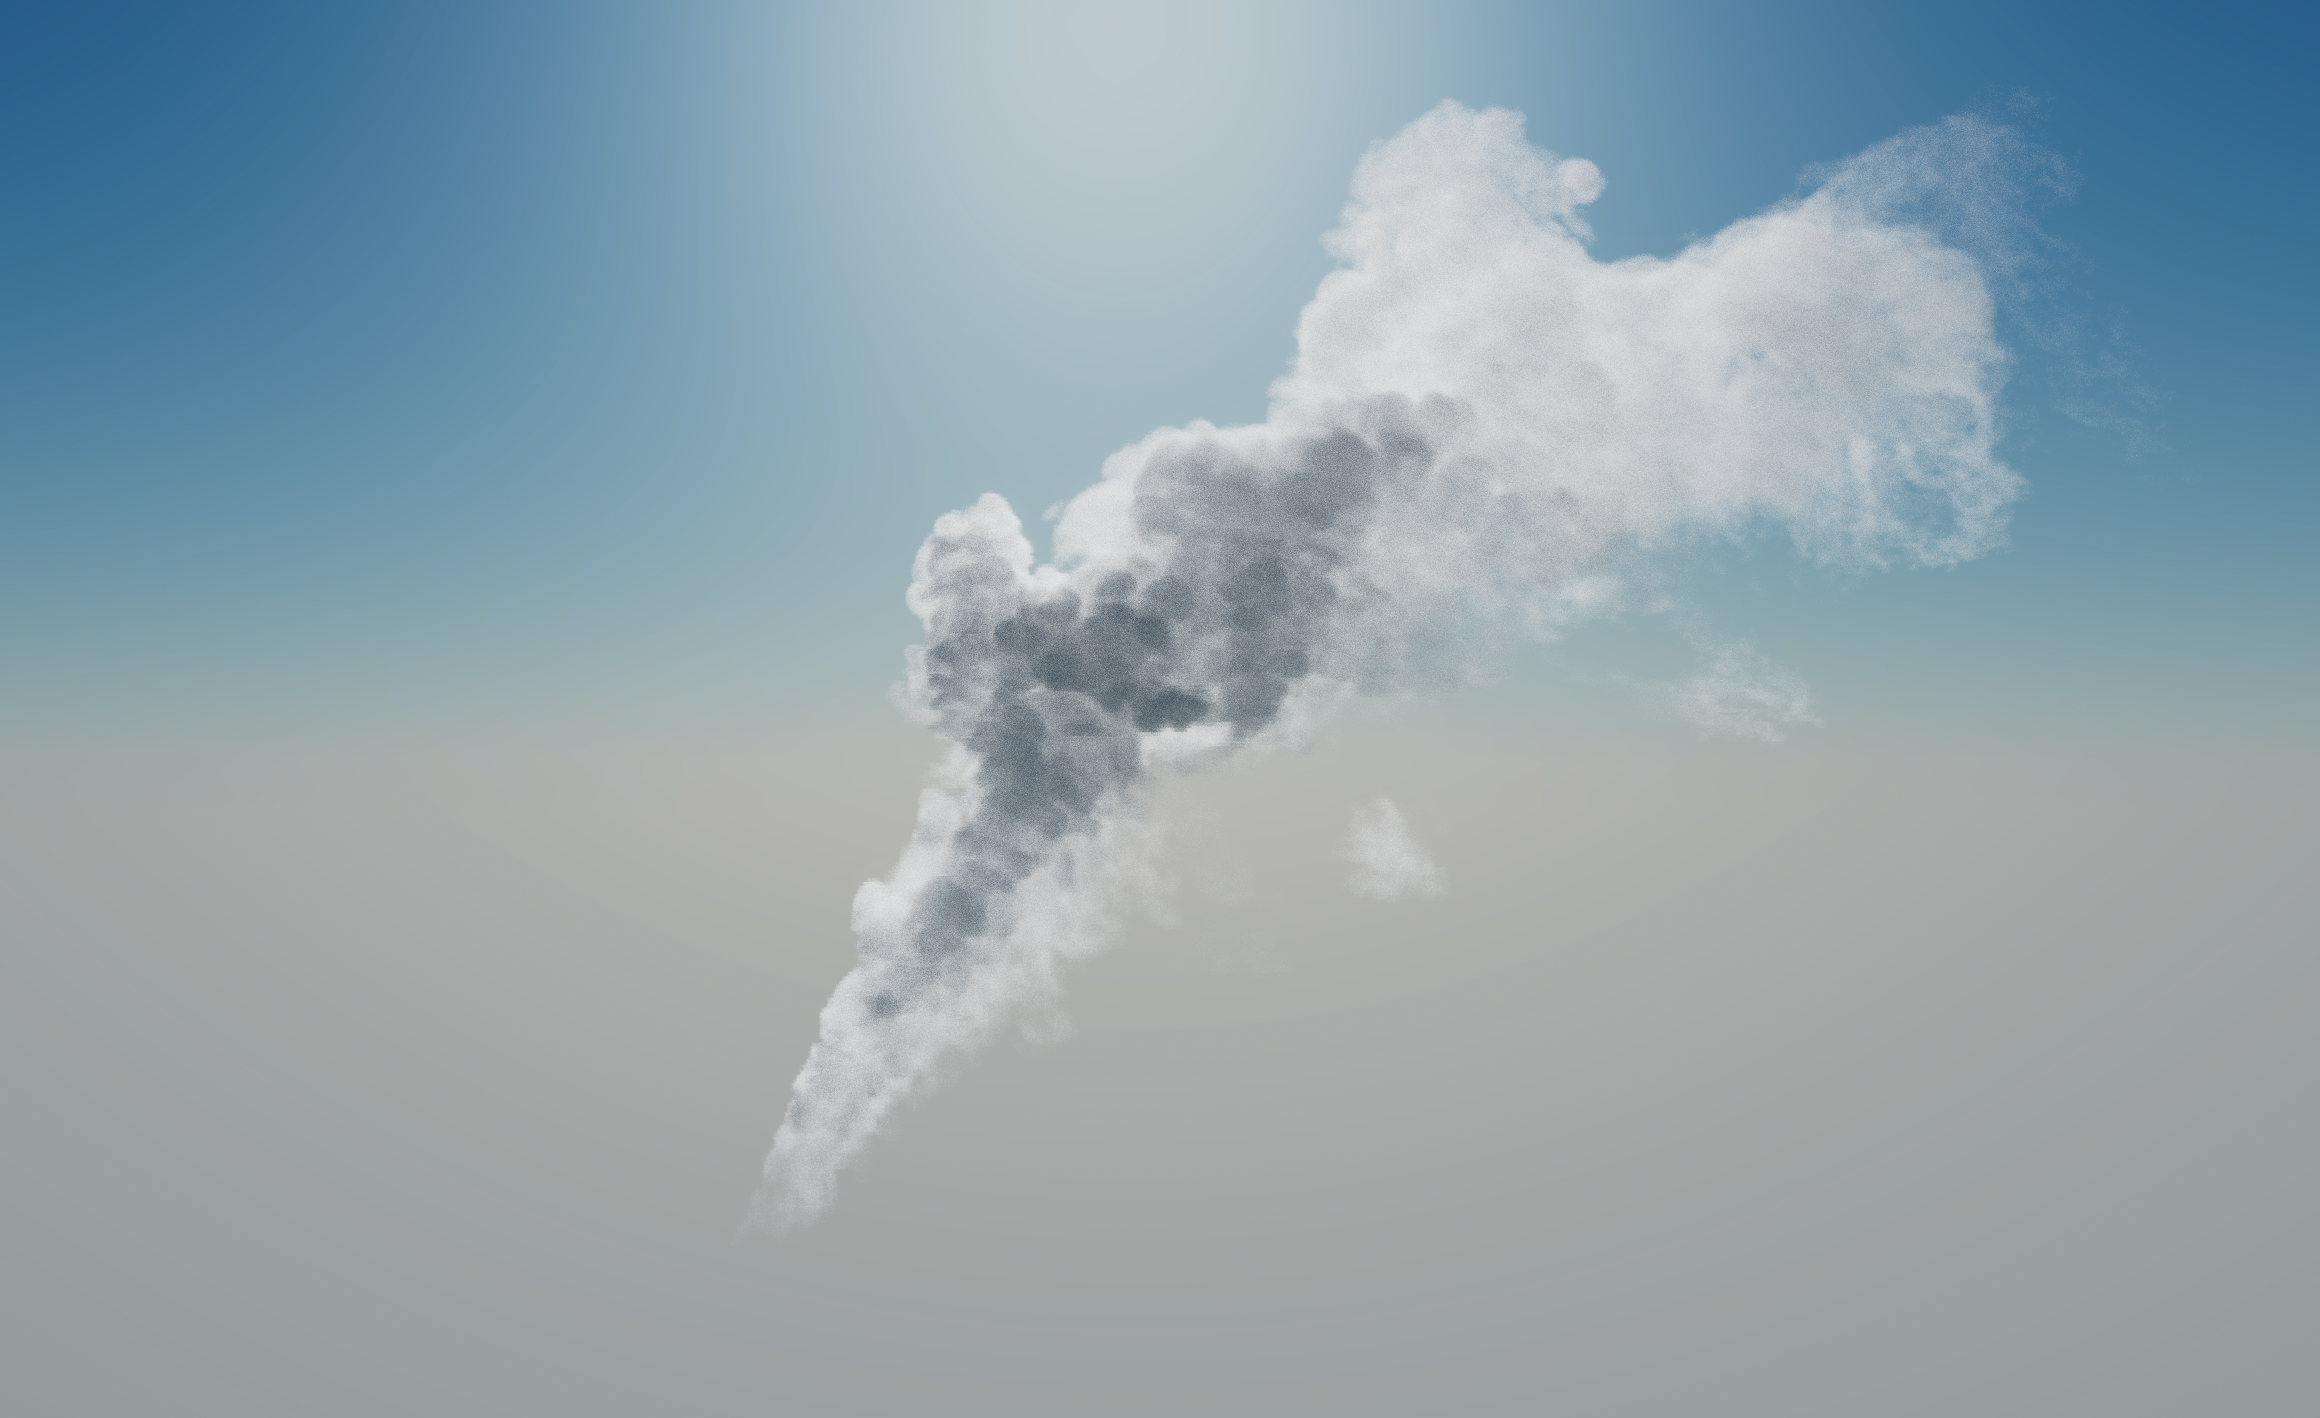
\includegraphics[width=4cm]{figures/chimney.png}\\
    \hline
    \textbf{shockwave} & 631,494,157 & [732, 140, 729] & 50 & 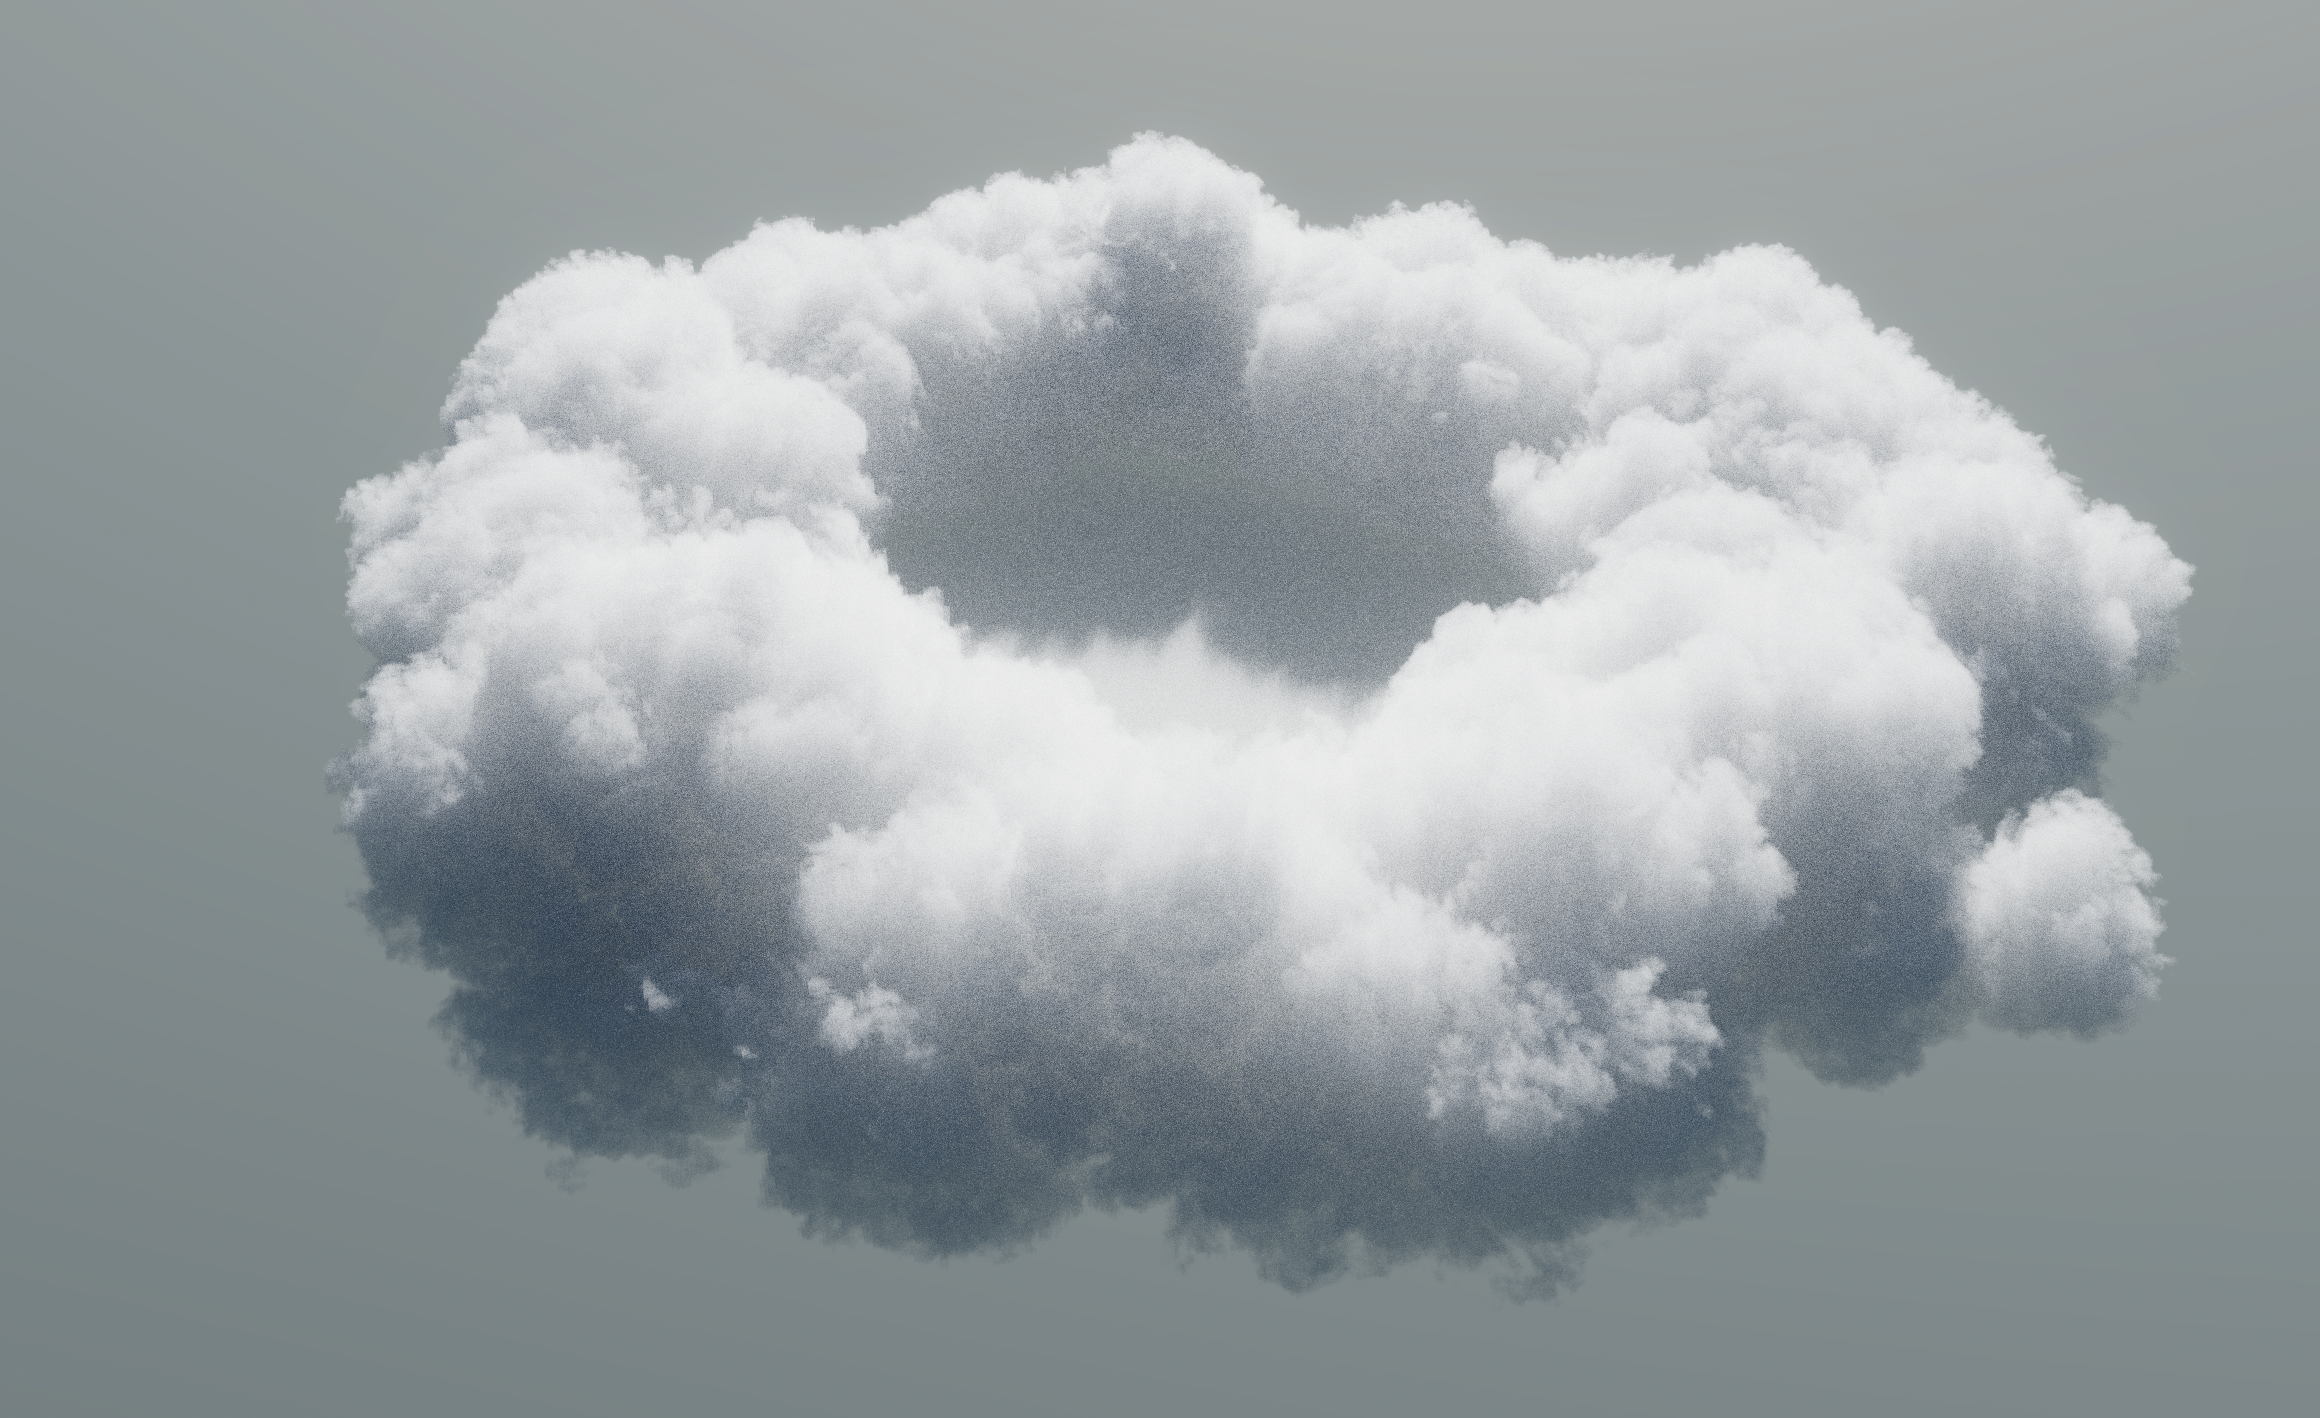
\includegraphics[width=4cm]{figures/shockwave.png}\\
    \hline
    \end{tabularx}
    \caption{The used volume models for our results. Bunny, armadillo and dragon consist of only the bounding edge of the volume. Cloud pack, chimney and shockwave contain multiple animation frames and thus can make use of delta compression. The voxels column indicates the number of non-zero voxels in the base model. All renders are done using the Breda framework using 1000 samples per pixel. }
    \label{tab:data-summary}
\end{table}


\subsection{Tree size} \label{results:tree_size}
As described in section \ref{approach:flipbook_animations}, we put our focus on compressing the voxel data instead of our tree structure size. This results in long animation sequences having large trees.  

\begin{table}[htbp]
    \centering
    \caption{Data Summary}
    \label{tab:data-summary}
    \begin{tabularx}{\textwidth}{|c|c|c|c|c|c|c|c|c|}
    \hline
    \textbf{Dataset} & \textbf{Total Voxels} & \textbf{Axis Sizes} & \textbf{L1 Nodes} & \textbf{L2 Nodes} & \textbf{L3 Nodes} & \textbf{Bricks} & \textbf{Total Size} \\
    \hline
    \textbf{fire} & 4,458,790 & [160, 363, 152] & 1 & 32,768 & 65,536 & 65,536 & 28MB & 1 \\
    \hline
    \textbf{bunny} & 5,513,993 & [627, 620, 488] & 1 & 32,768 & 307,200 & 65,536 & 46MB & 1 \\
    \hline
    \textbf{bunny cloud} & 19,210,271 & [576, 571, 437] & 1 & 32,768 & 303,104 & 131,072 & 54MB & 1 \\
    \hline
    \textbf{armadillo} & 22,734,512 & [1,275, 1,518, 1,159] & 1 & 32,768 & 1,339,392 & 131,072 & 125MB & 1 \\
    \hline
    \textbf{dragon} & 23,347,893 & [2,022, 910, 1,346] & 1 & 32,768 & 1,302,528 & 131,072 & 122MB & 1 \\
    \hline
    \textbf{cloud pack} & 49,869,596 & [349, 178, 530] & 10 & 327,680 & 905,216 & 196,608 & 255MB & 10 \\
    \hline
    \textbf{disney cloud} & 188,358,293 & [993, 675, 1,224] & 1 & 32,768 & 1,007,616 & 327,680 & 127MB & 1 \\
    \hline
    \textbf{chimney} & 239,747,485 & [160, 350, 505] & 100 & 3,276,800 & 9,195,520 & 917,504 & 2.434GB & 100 \\
    \hline
    \textbf{shockwave} & 631,494,157 & [732, 140, 729] & 50 & 1,638,400 & 9,658,368 & 1,900,544 & 1.746GB & 50 \\
    \hline
    \end{tabularx}
\end{table}

\subsection{Block compression} \label{results:block_compression}

\begin{figure}[H]
    \centering
    %\subfloat[]{
    %    \includegraphics[width=0.45\textwidth]{}
    %}
    %\hfill
    %\subfloat[]{
    %    \includegraphics[width=0.45\textwidth]{}
    %}

    \caption{} \label{fig:implementation:compression:bc}
\end{figure}
\subsection{Clustering} \label{results:clustering}


\begin{figure}[H]
    \centering
    \subfloat[]{
        \includegraphics[width=0.45\textwidth]{figures/pre_clustered_memory.png} \label{fig:implementation:compression:pre_cluster}
    }
    \hfill
    \subfloat[]{
        \includegraphics[width=0.45\textwidth]{figures/post_clustered_memory.png} \label{fig:implementation:compression:post_cluster}
    }
    \caption{The results of our clustering compression technique. All of these results use Bc7 encoding. Figure \ref{fig:implementation:compression:pre_cluster} shows a slice out of the voxel brick data texture on the GPU. There are visible long chains of black or otherwise greyscale slices which means that these bricks are mostly homogeneous inside that brick. In Figure \ref{fig:implementation:compression:post_cluster} we again see a slice of the voxel brick data texture, but this time after running our clustering algorithm. There are visibly fewer patches greyscale bricks when compared to figure \ref{fig:implementation:compression:pre_cluster}. This shows us that we are actually removing bricks which are homogeneous, and keeping unique nodes.} \label{fig:implementation:compression:cluster}
\end{figure}